\section{Algorithm Testing}
\label{sec:algorithm_testing}

Now that the algorithm has been implemented, we can proceed presenting at first the test environment that have been used to test them and then the results of the tests.

Figures \ref{fig:test_maps} show the four image maps used to test the algorithm.
Even if the images here below are of size 300x300, we preferred to scale down to 30x30 given that each pixel is then converted into a node of the graph and so to avoid huge graphs and long computation times.
Notice also that while the white areas are free space, the one marked in black or gray are to be considered as obstacles.
Finally, the green dot is the starting point of the vehicle, while the red one is the goal.

\begin{figure}[H]
    \centering
    \frame{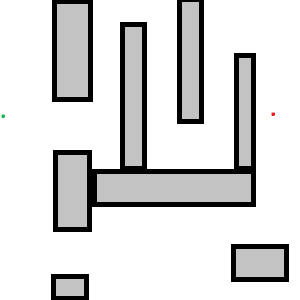
\includegraphics[width=0.48\textwidth]{./img/01.png}}
    \hspace{6pt}
    \frame{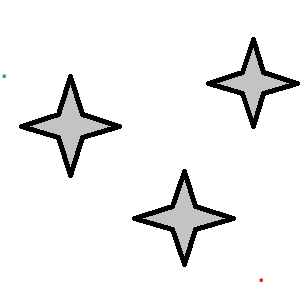
\includegraphics[width=0.48\textwidth]{./img/02.png}}

    \vspace{11pt}

    \frame{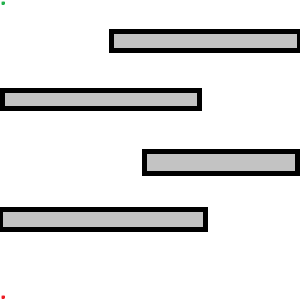
\includegraphics[width=0.48\textwidth]{./img/03.png}}
    \hspace{6pt}
    \frame{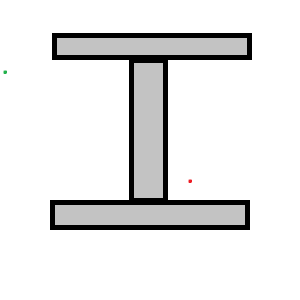
\includegraphics[width=0.48\textwidth]{./img/04.png}}
    \caption{Test maps used for the algorithm testing.}
    \label{fig:test_maps}
\end{figure}

In the following, results obtained running both the A* and the Dijkstra algorithms on each of the four maps are presented.

The plotting of both the (geometrical) connected graph and the best path found is also shown.
Notice that each test case has been run allowing or disabling the diagonal movement of the vehicle, which can be achieved during the graph generation phase modifying the connection of the nodes.

Tables presenting the main metrics of the tests are also shown.
The metrics are the following:

\begin{itemize}
    \item \textbf{Elapsed time}: here only the time needed to run the searching algorithm is considered (i.e. we are excluding both the generation of the graph and the plotting of the results);
    \item \textbf{Nodes analyzed}: number of nodes analyzed (visited) before reaching the goal;
    \item \textbf{Path length}: length of the path found by the algorithm. This also correspond to the path cost, given that the cost of each edge is equal to its geometrical length.
\end{itemize}



\subsection{Map 1}
\label{subsec:map_1}

Results obtained running the A* and Dijkstra algorithms on Map 1 are shown in Figures \ref{fig:map_1_results} and Table \ref{tab:map_1_results}.
About the figures, the upper row shows the graph generated running the Dijkstra algorithm while the lower one shows the graph generated running the A* algorithm.
The left column shows the graph generated allowing only orthogonal movements, while the right one shows the graph generated allowing also diagonal movements.
The path found by the algorithm is shown in red, while the graph is shown in black.

\begin{figure}[H]
    \centering
    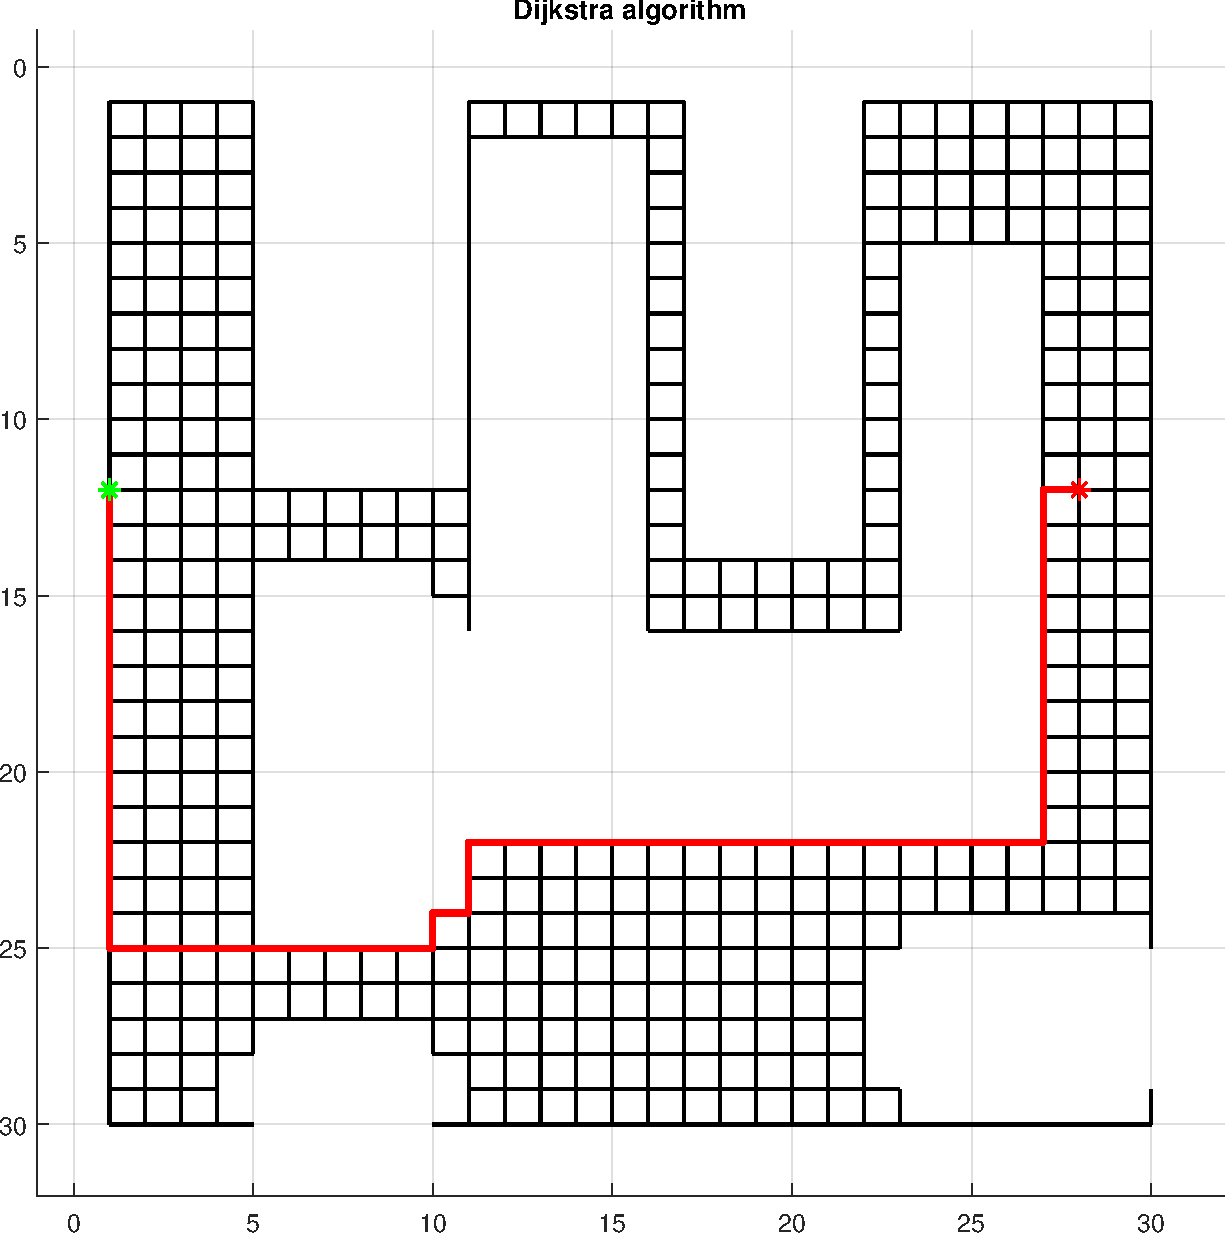
\includegraphics[width=0.48\textwidth]{./img/MATLAB/01_dijkstra_orthogonal.pdf}
    \hspace{6pt}
    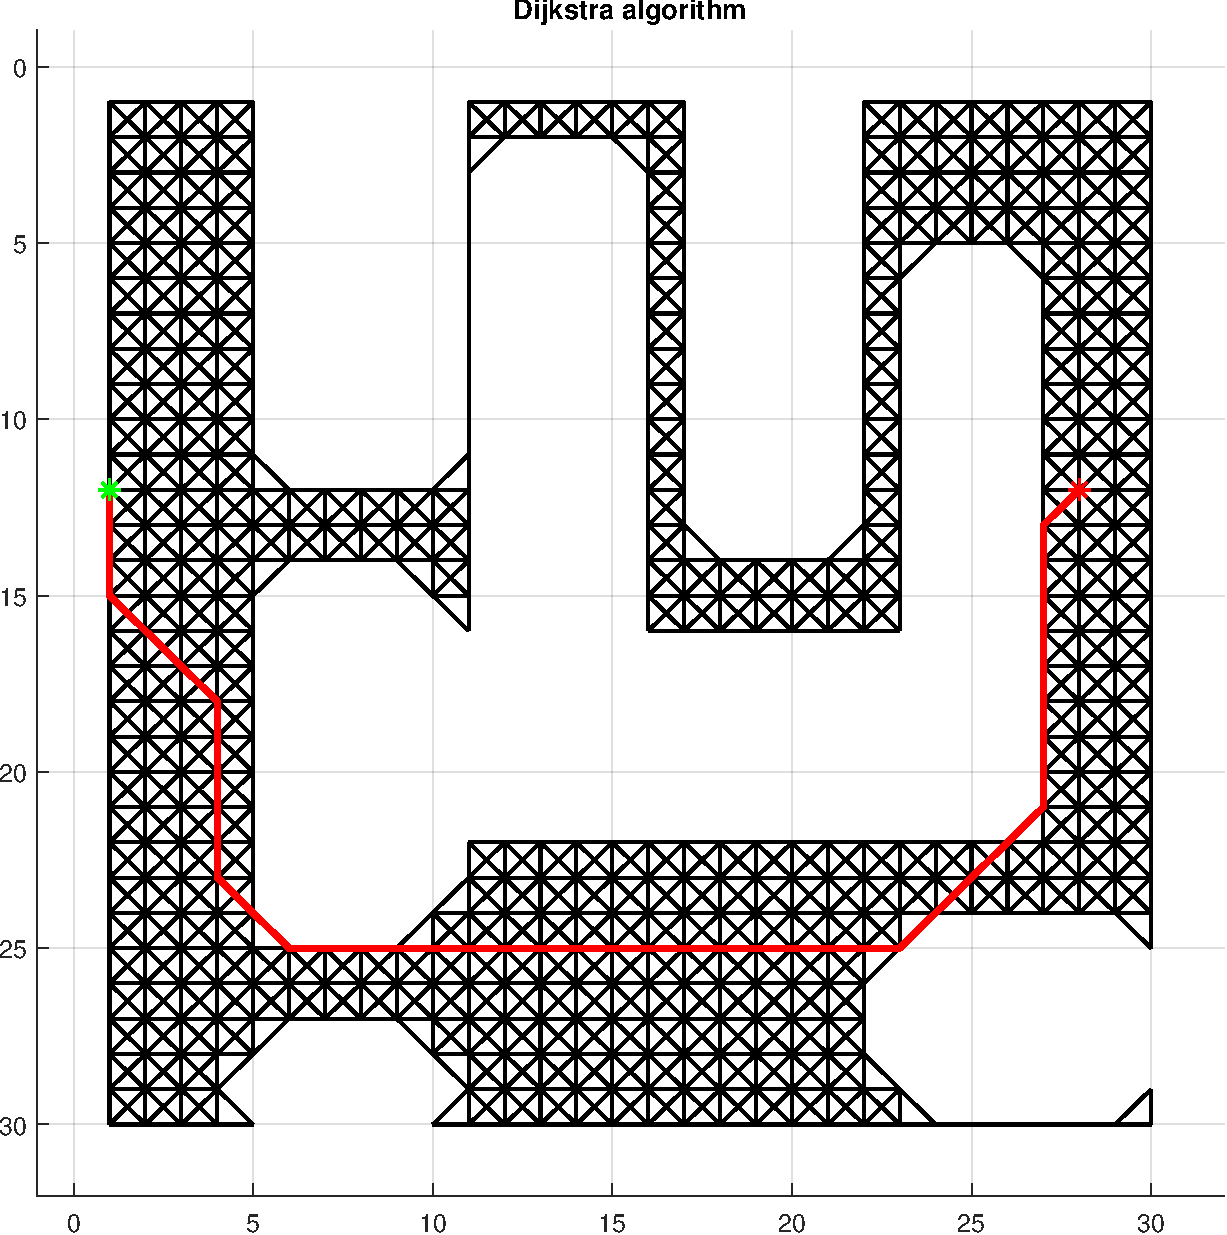
\includegraphics[width=0.48\textwidth]{./img/MATLAB/01_dijkstra_diagonal.pdf}

    \vspace{11pt}

    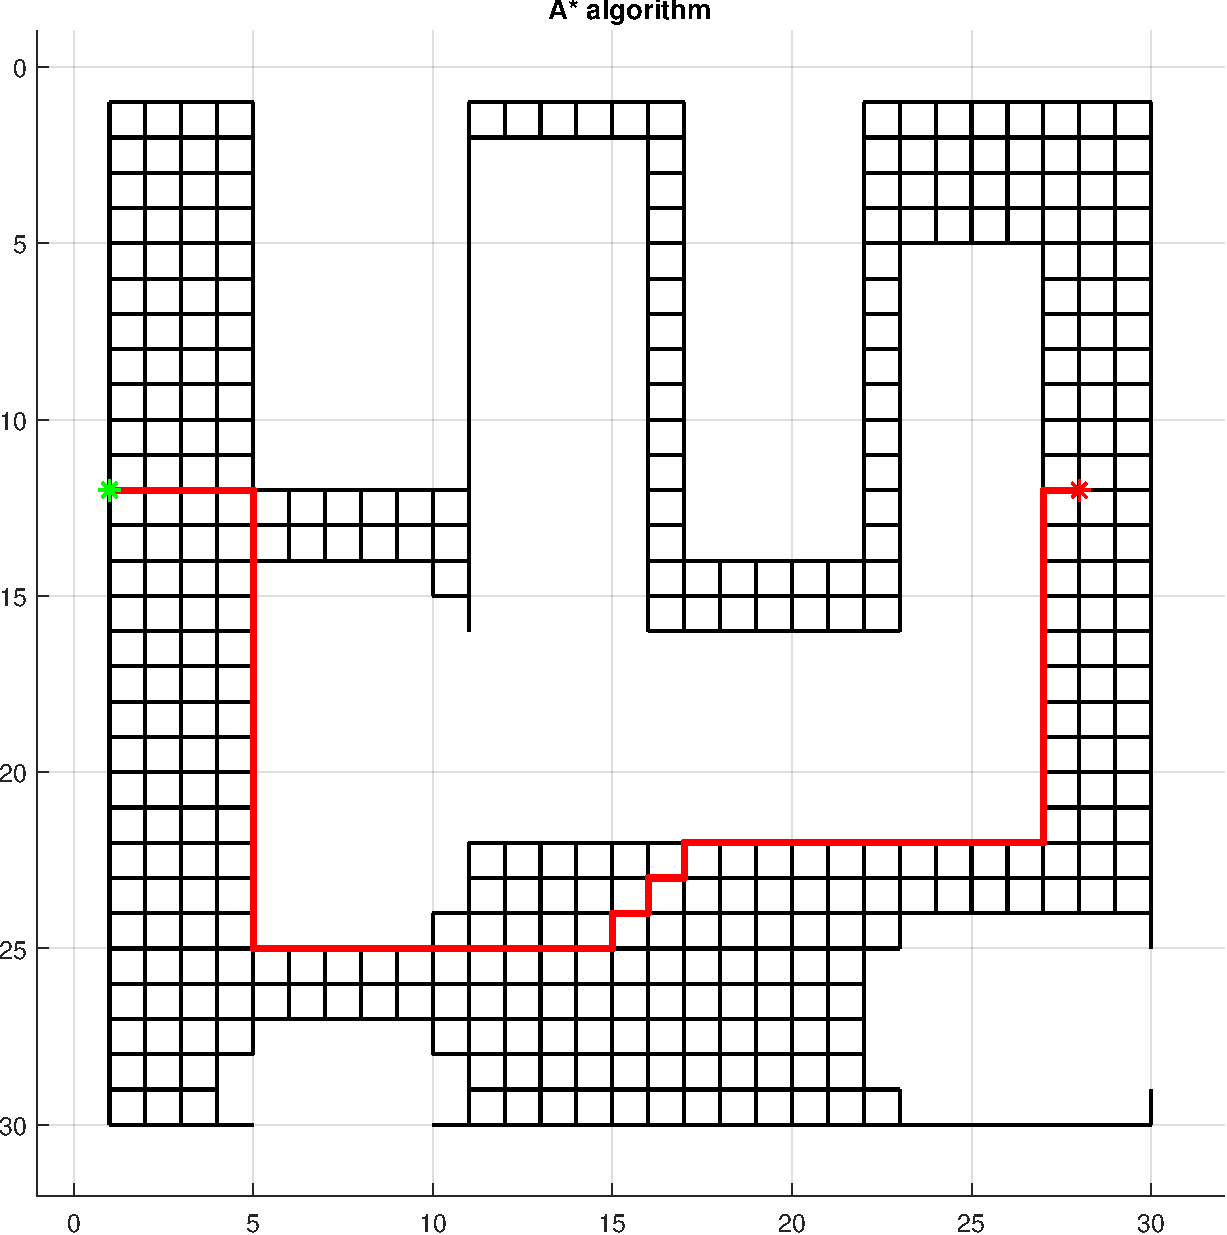
\includegraphics[width=0.48\textwidth]{./img/MATLAB/01_astar_orthogonal.pdf}
    \hspace{6pt}
    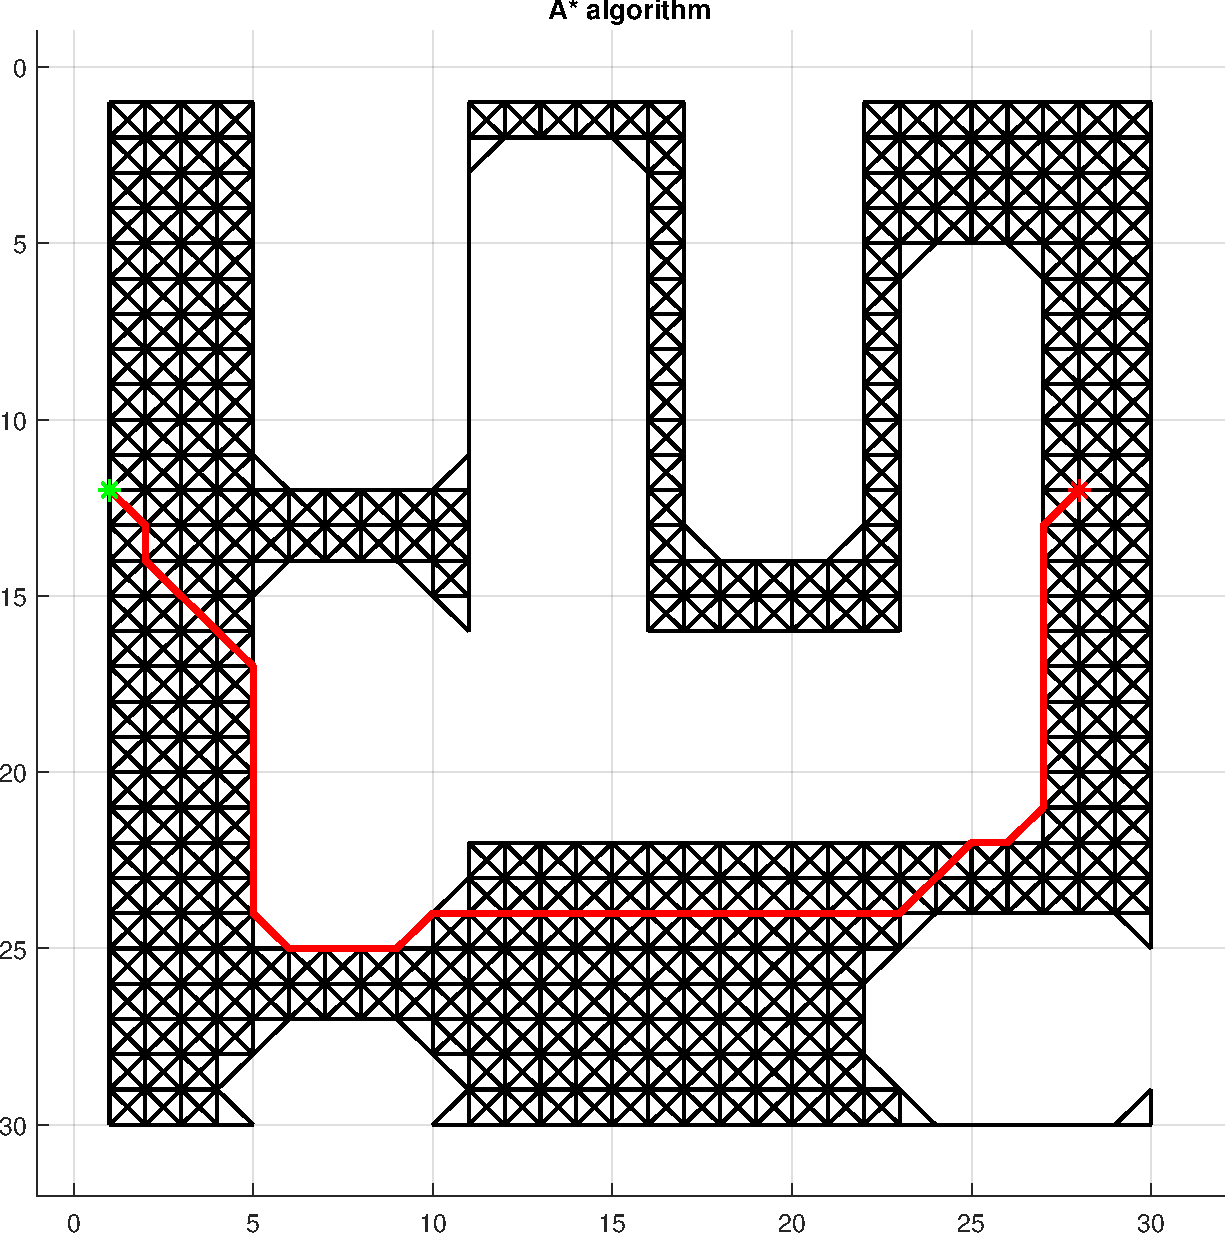
\includegraphics[width=0.48\textwidth]{./img/MATLAB/01_astar_diagonal.pdf}
    \caption{Map 1: Graph and path found by the algorithms.}
    \label{fig:map_1_results}
\end{figure}

\begin{table}[H]
    \centering
    \begin{tabular}{|c|c|c|c|c|c|}
        \hline
        \textbf{Algorithm}        & \textbf{Diagonal} & \textbf{Elapsed time (ms)} & \textbf{Nodes analyzed} & \textbf{Path length (m)} \\
        \hline
        \multirow{2}{*}{Dijkstra} & No                & 624                        & 456                     & 53                       \\
                                  & Yes               & 1592                       & 453                     & 47                       \\
        \hline
        \multirow{2}{*}{A*}       & No                & 339                        & 378                     & 53                       \\
                                  & Yes               & 1227                       & 339                     & 47                       \\
        \hline
    \end{tabular}
    \caption{Map 1: Results of the tests.}
    \label{tab:map_1_results}
\end{table}

From the results presented in Table \ref{tab:map_1_results} and in Figure \ref{fig:map_1_results}, we can already notice that while the cost of the path found by the two algorithms is equivalent, the number of nodes considered by the A* algorithm is significantly lower than the one considered by the Dijkstra algorithm.
This behavior is expected due to the use of the heuristic function to guide the search of the A* algorithm.
The advantage in terms of computational time is also evident, with the A* algorithm outperforming the Dijkstra algorithm.



\subsection{Map 2}
\label{subsec:map_2}

Results obtained running the A* and Dijkstra algorithms on Map 2 are shown in Figures \ref{fig:map_2_results} and Table \ref{tab:map_2_results}.
The same layout of the previous map is used for the figures and the same metrics are used for the table.

\begin{figure}[H]
    \centering
    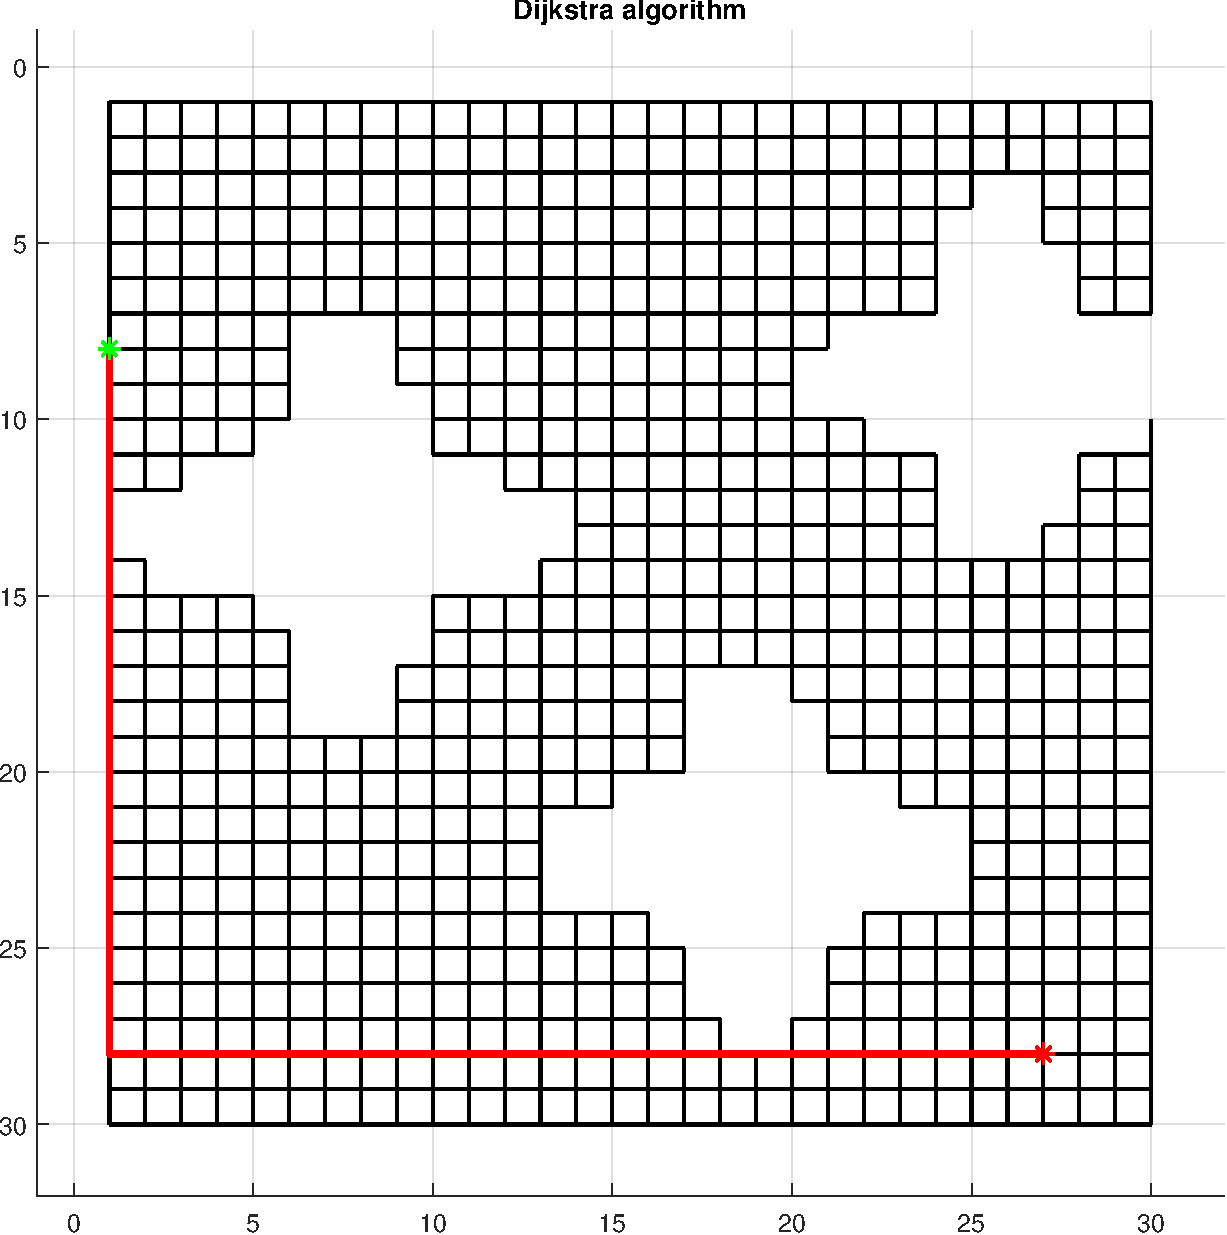
\includegraphics[width=0.48\textwidth]{./img/MATLAB/02_dijkstra_orthogonal.pdf}
    \hspace{6pt}
    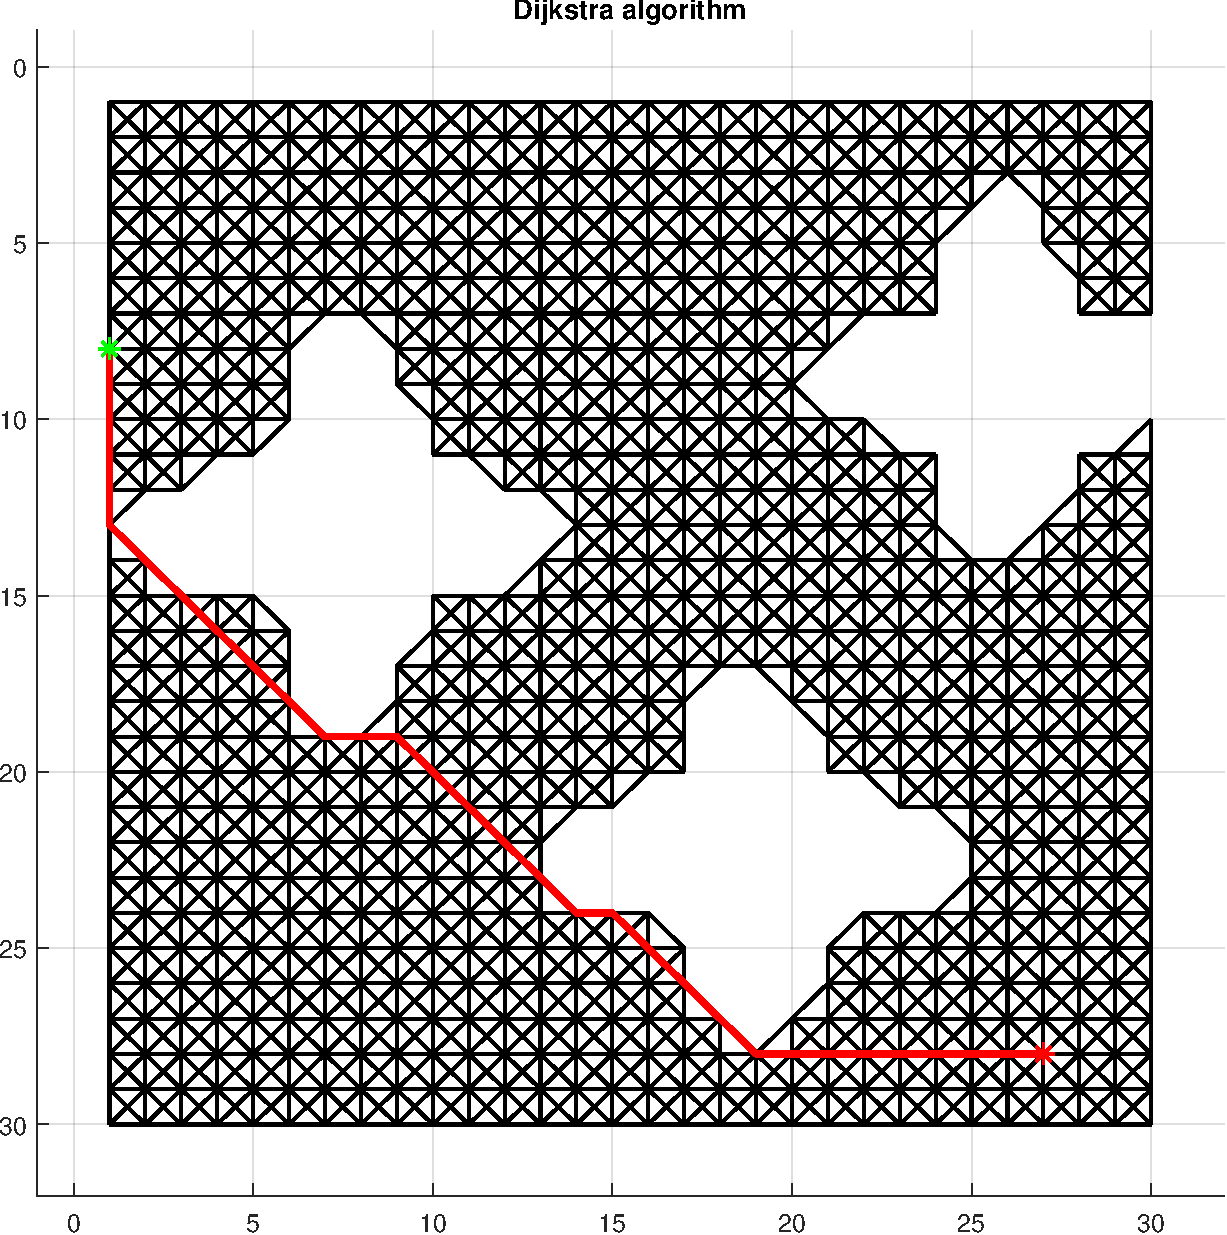
\includegraphics[width=0.48\textwidth]{./img/MATLAB/02_dijkstra_diagonal.pdf}

    \vspace{11pt}

    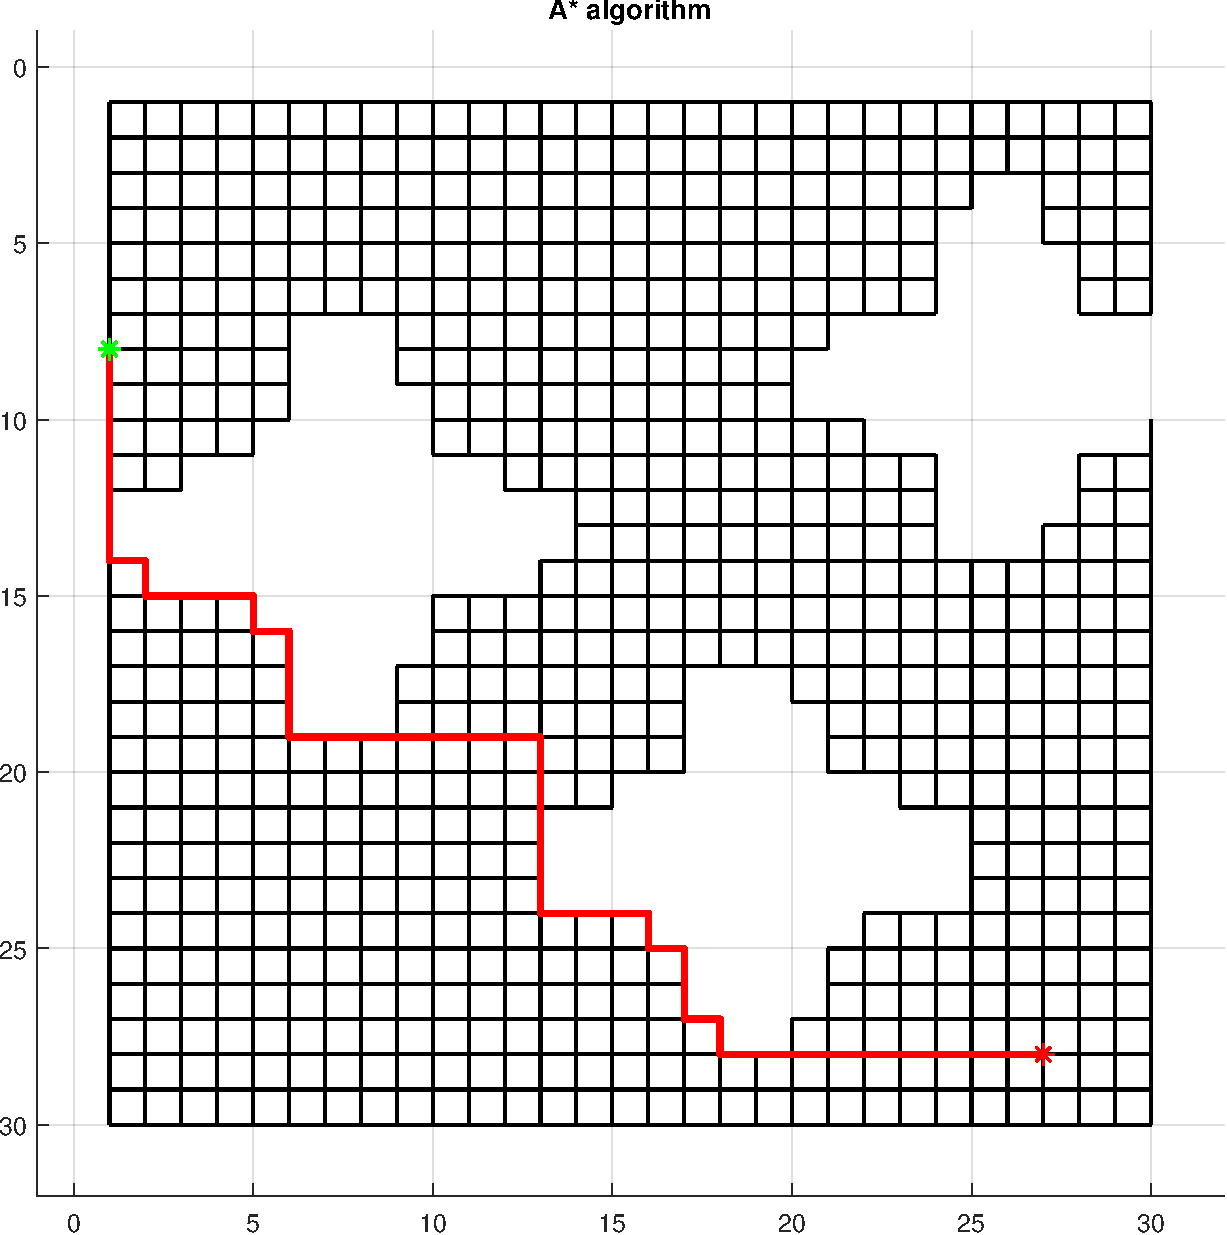
\includegraphics[width=0.48\textwidth]{./img/MATLAB/02_astar_orthogonal.pdf}
    \hspace{6pt}
    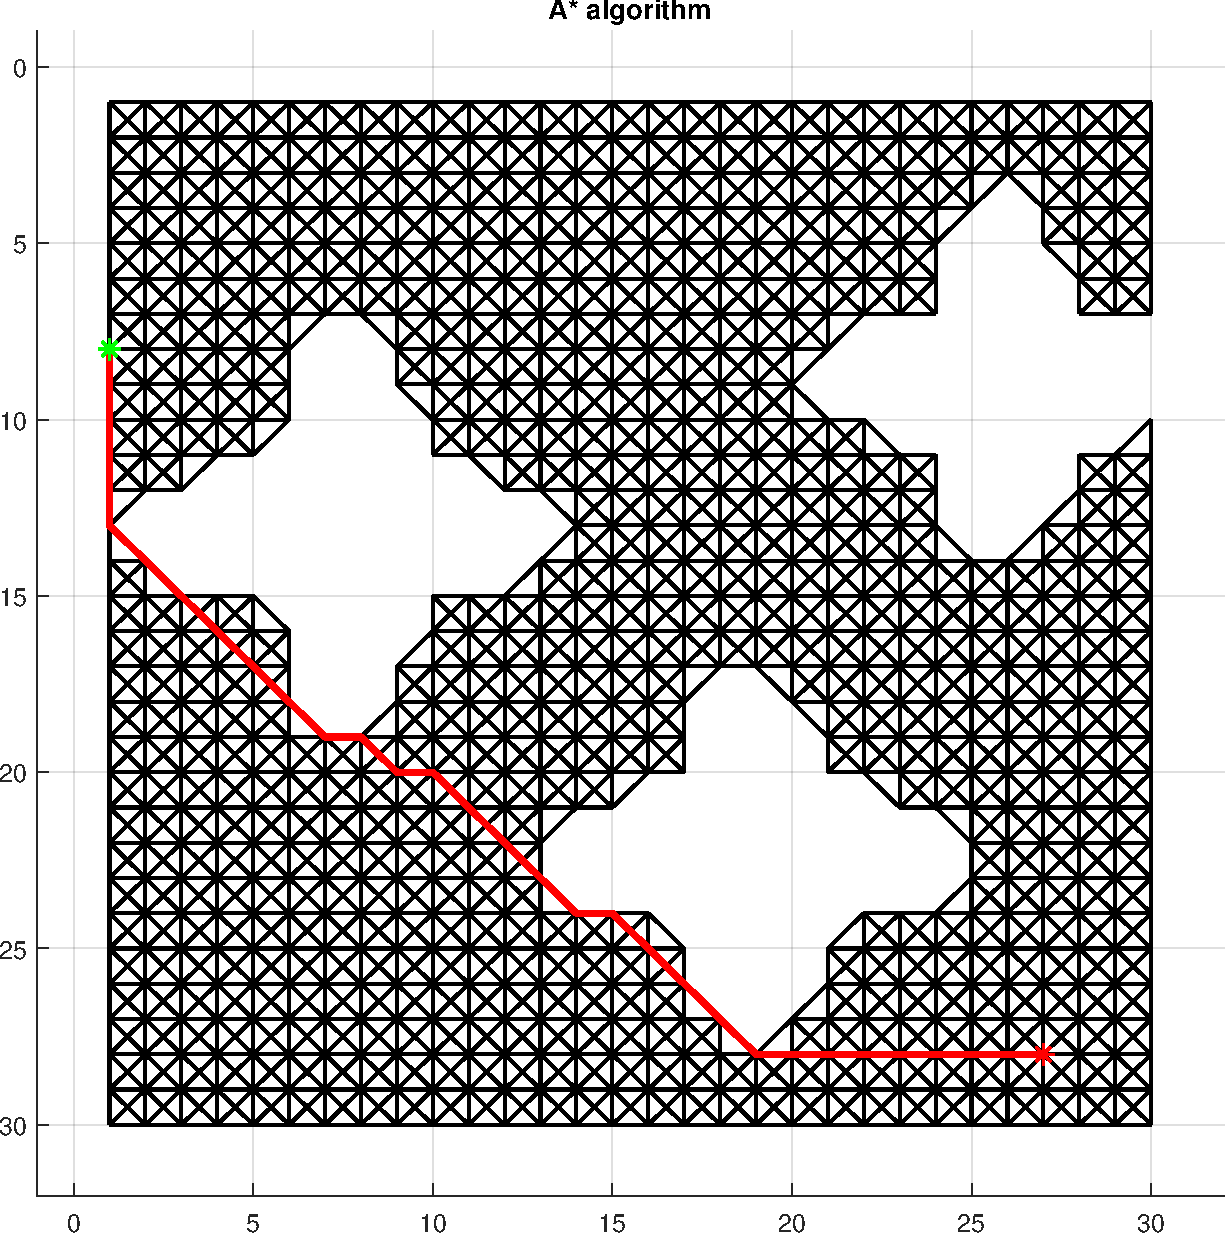
\includegraphics[width=0.48\textwidth]{./img/MATLAB/02_astar_diagonal.pdf}
    \caption{Map 2: Graph and path found by the algorithms.}
    \label{fig:map_2_results}
\end{figure}

\begin{table}[H]
    \centering
    \begin{tabular}{|c|c|c|c|c|c|}
        \hline
        \textbf{Algorithm}        & \textbf{Diagonal} & \textbf{Elapsed time (ms)} & \textbf{Nodes analyzed} & \textbf{Path length (m)} \\
        \hline
        \multirow{2}{*}{Dijkstra} & No                & 1009                       & 731                     & 46                       \\
                                  & Yes               & 3963                       & 742                     & 37                       \\
        \hline
        \multirow{2}{*}{A*}       & No                & 732                        & 490                     & 46                       \\
                                  & Yes               & 1434                       & 233                     & 37                       \\
        \hline
    \end{tabular}
    \caption{Map 2: Results of the tests.}
    \label{tab:map_2_results}
\end{table}

Similarly to the previous map, the results presented in Table \ref{tab:map_2_results} and in Figure \ref{fig:map_2_results} show that while the cost of the path found by the two algorithms is equivalent, the number of nodes considered by the A* algorithm is significantly lower than the one considered by the Dijkstra algorithm.
Similar conclusions can be drawn in terms of computational time and performance of the two algorithms.

As an additional note, in this case we can also appreciate that the number of analyzed nodes by A* is significantly lower than the one analyzed by Dijkstra, particularly in case of diagonal movements.
This is, however, expected.
Looking at the final path, we observe that is almost equivalent to the diagonal connecting ideally the start and goal points.
This means that the heuristic function used by A* is even more effective in this case, given that very few obstacles are present along the optimal path designed by the heuristic function itself and so fewer death ends are encountered.
In other words, if the optimal path turns out to be a straight line connecting the start and goal points, the A* algorithm would analyze a number of nodes equal to the number of nodes along the straight line, while the Dijkstra algorithm would still analyze a much larger number of nodes given that no information is used to guide the search.


\subsection{Map 3}
\label{subsec:map_3}

Results obtained running the A* and Dijkstra algorithms on Map 3 are shown in Figures \ref{fig:map_3_results} and table.
The same layout of the previous map is used for the figures and the same metrics are used for the table.

\begin{figure}[H]
    \centering
    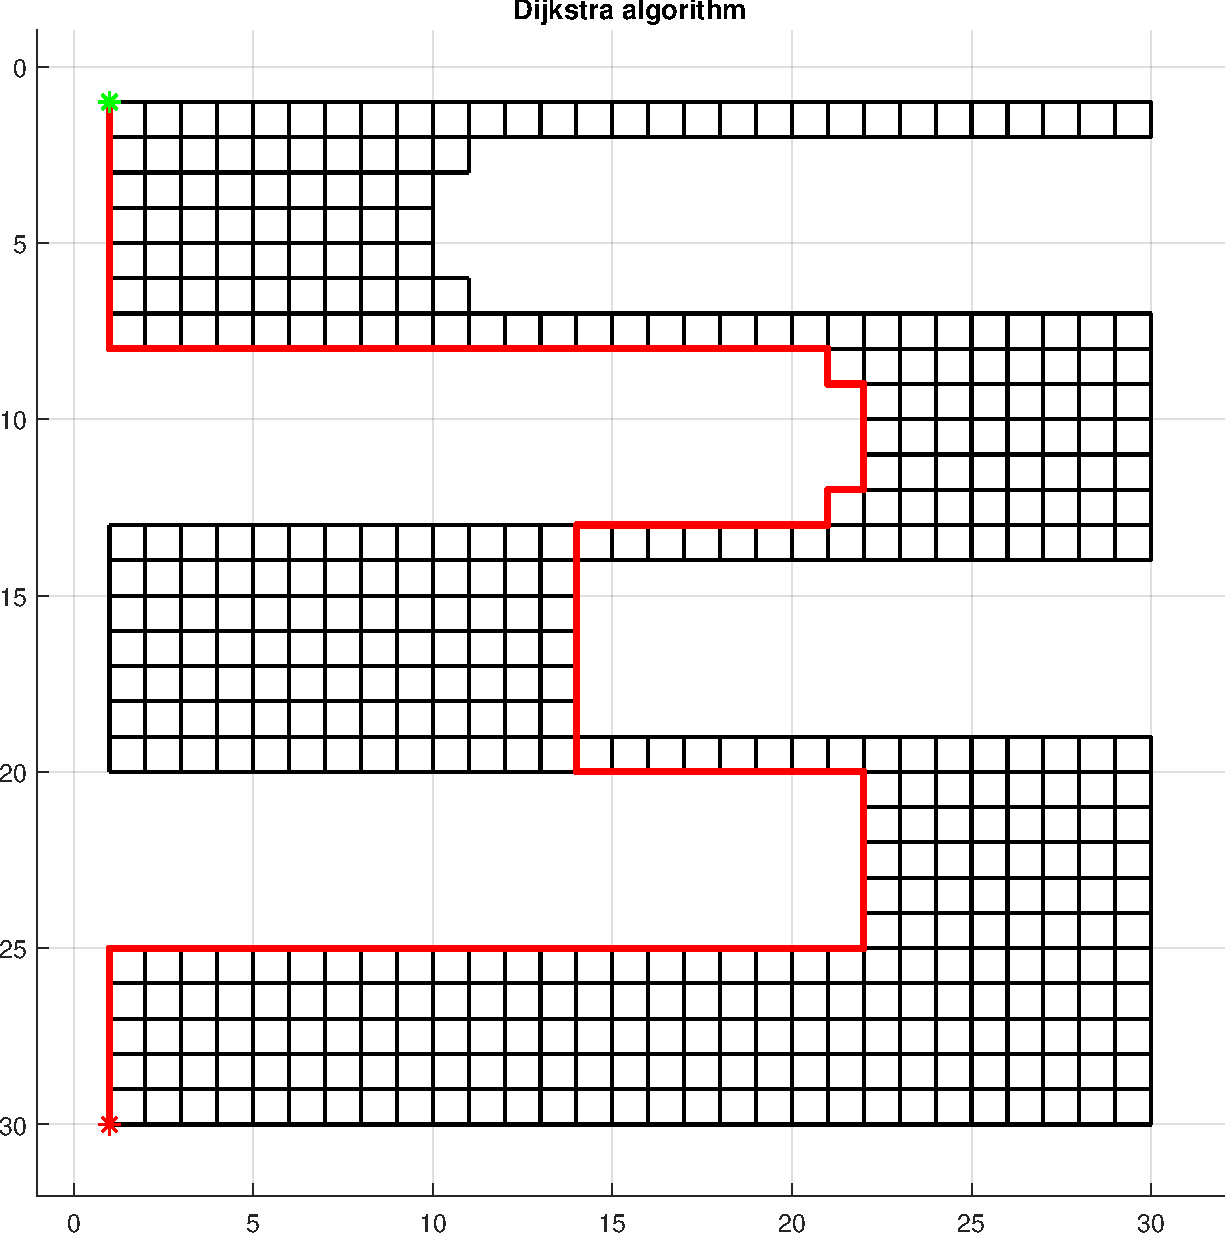
\includegraphics[width=0.48\textwidth]{./img/MATLAB/03_dijkstra_orthogonal.pdf}
    \hspace{6pt}
    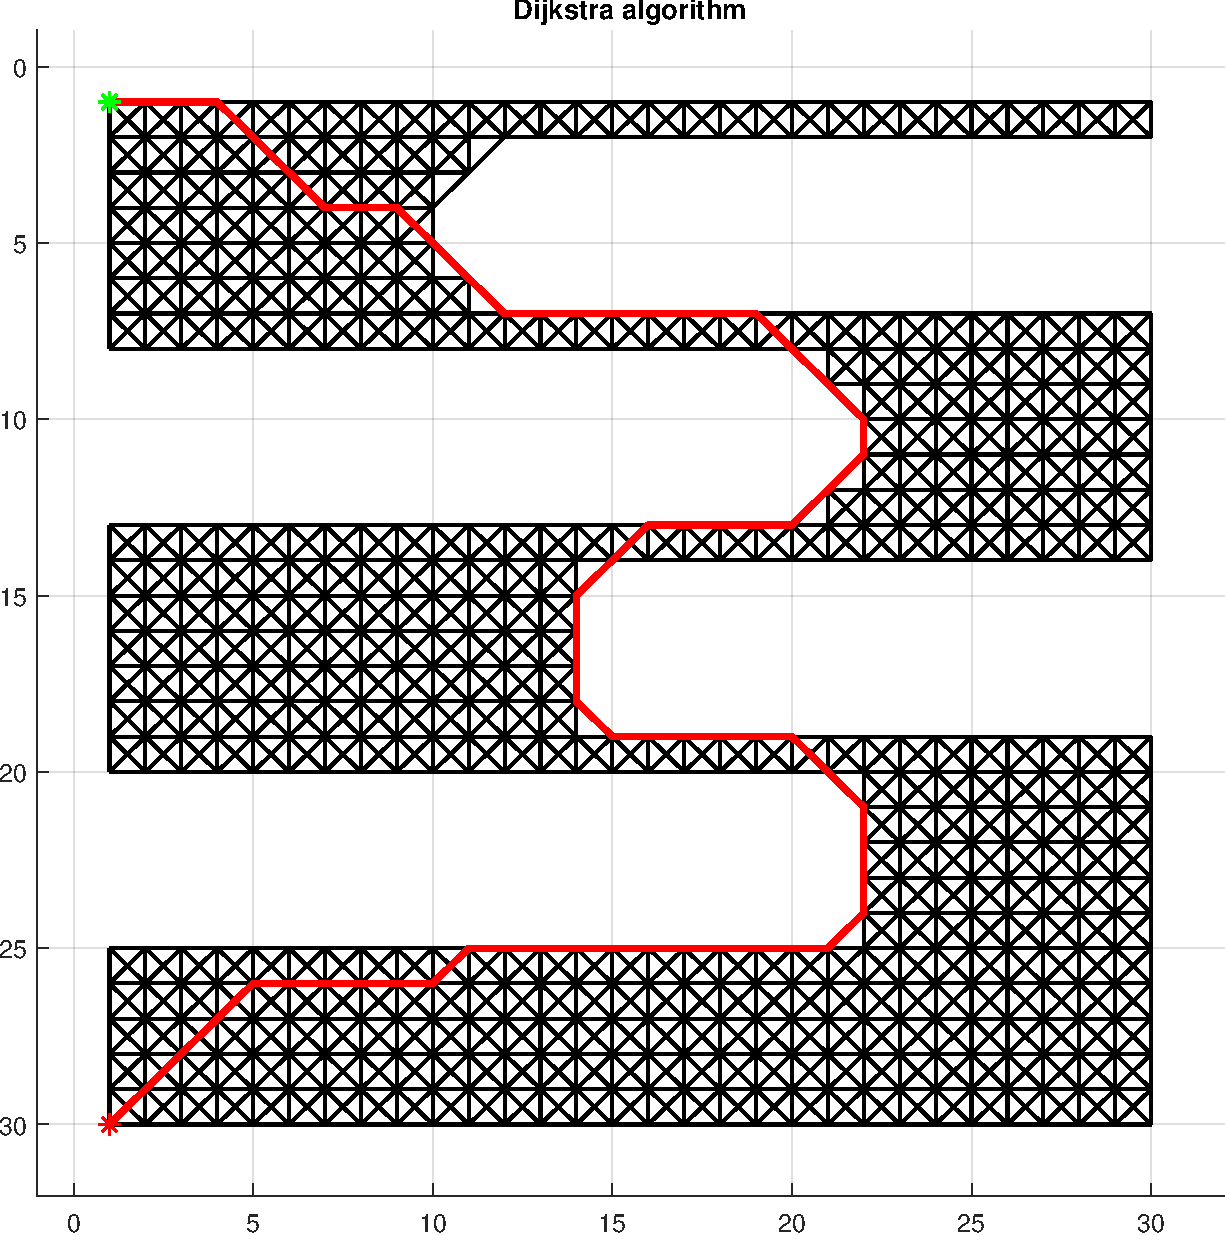
\includegraphics[width=0.48\textwidth]{./img/MATLAB/03_dijkstra_diagonal.pdf}

    \vspace{11pt}

    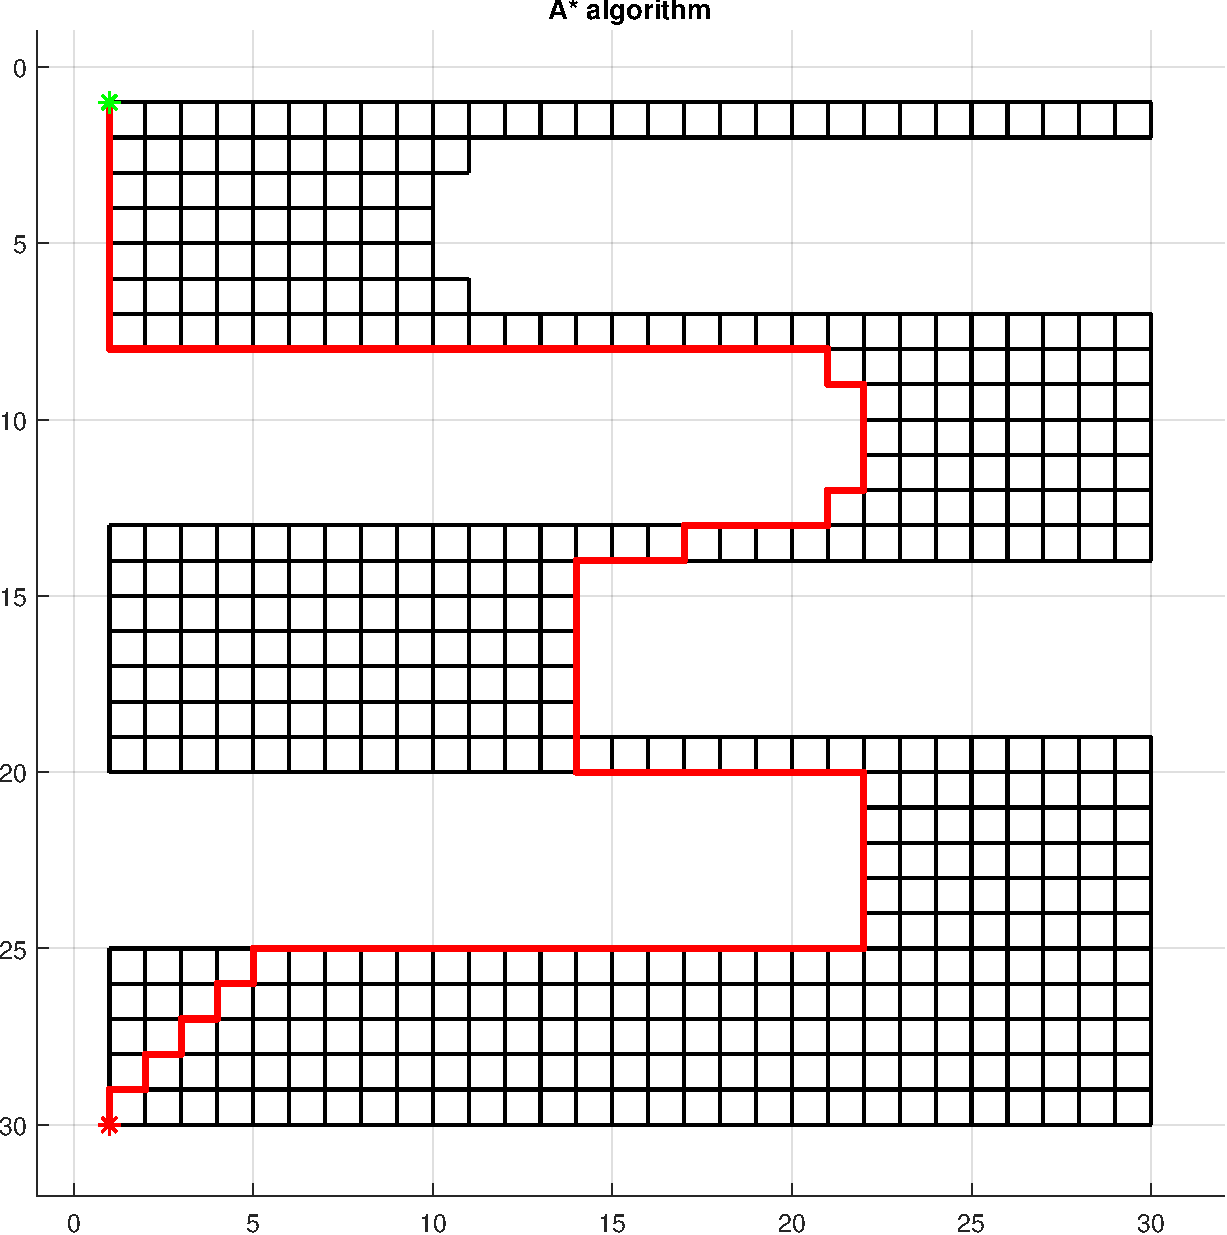
\includegraphics[width=0.48\textwidth]{./img/MATLAB/03_astar_orthogonal.pdf}
    \hspace{6pt}
    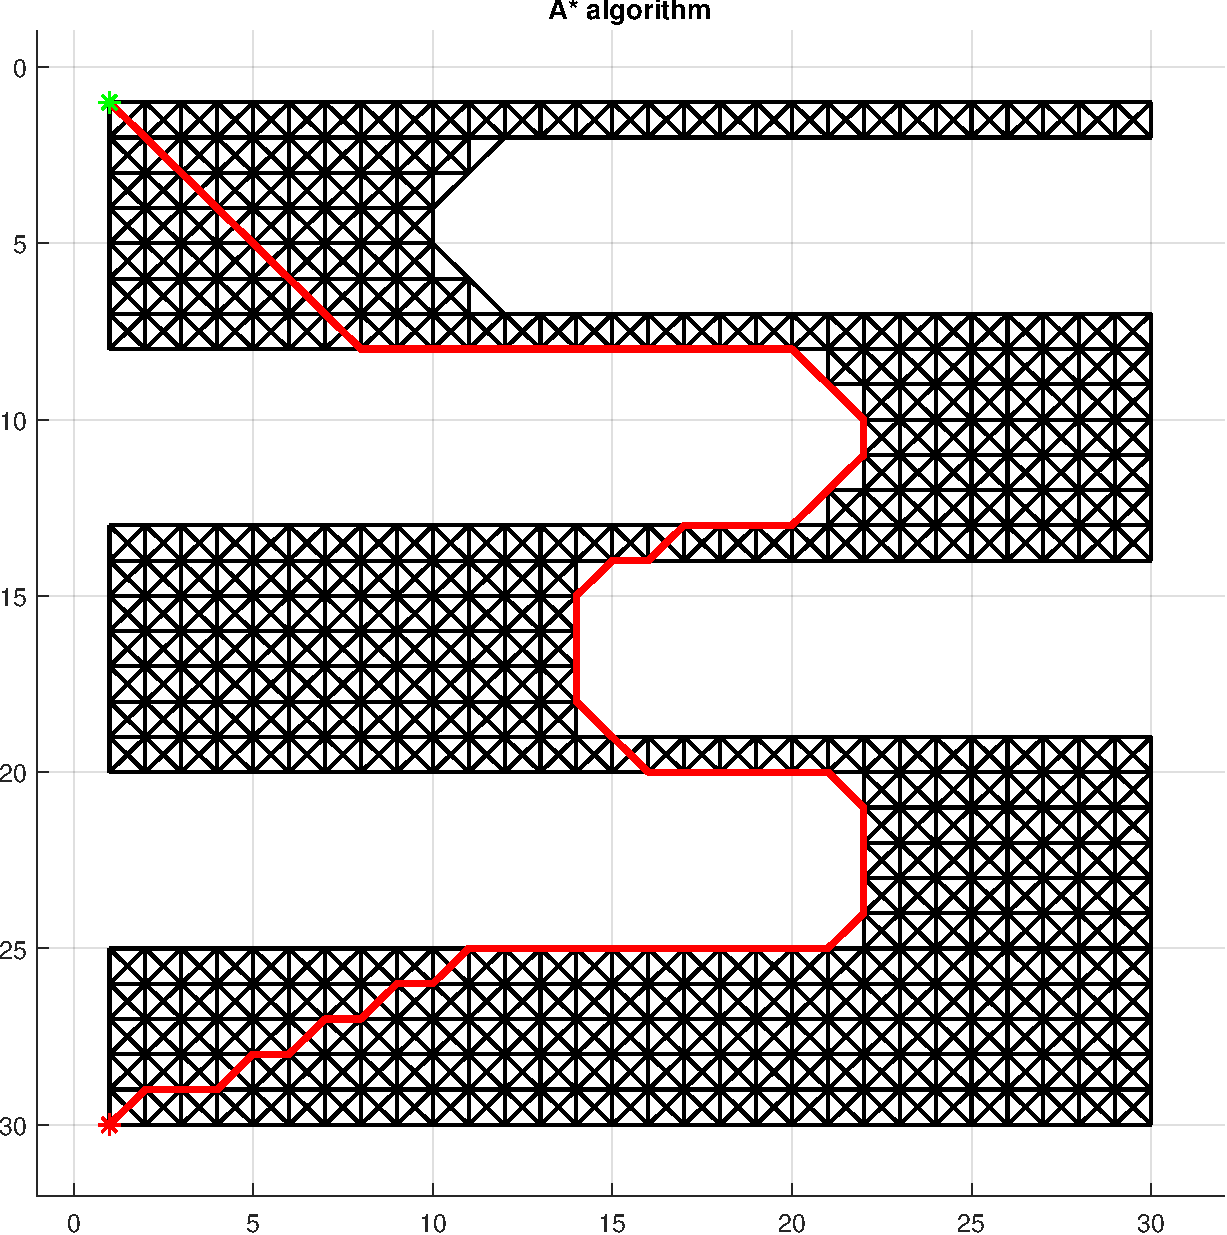
\includegraphics[width=0.48\textwidth]{./img/MATLAB/03_astar_diagonal.pdf}
    \caption{Map 3: Graph and path found by the algorithms.}
    \label{fig:map_3_results}
\end{figure}

\begin{table}[H]
    \centering
    \begin{tabular}{|c|c|c|c|c|c|}
        \hline
        \textbf{Algorithm}        & \textbf{Diagonal} & \textbf{Elapsed time (ms)} & \textbf{Nodes analyzed} & \textbf{Path length (m)} \\
        \hline
        \multirow{2}{*}{Dijkstra} & No                & 567                        & 592                     & 87                       \\
                                  & Yes               & 2461                       & 592                     & 74                       \\
        \hline
        \multirow{2}{*}{A*}       & No                & 496                        & 497                     & 87                       \\
                                  & Yes               & 1780                       & 452                     & 74                       \\
        \hline
    \end{tabular}
    \caption{Map 3: Results of the tests.}
    \label{tab:map_3_results}
\end{table}

Again, similar considerations as before can be drawn from the results presented in Table \ref{tab:map_3_results} and in Figure \ref{fig:map_3_results}.


\subsection{Map 4}
\label{subsec:map_4}

Results obtained running the A* and Dijkstra algorithms on Map 4 are shown in Figures \ref{fig:map_4_results} and table.
The same layout of the previous map is used for the figures and the same metrics are used for the table.

\begin{figure}[H]
    \centering
    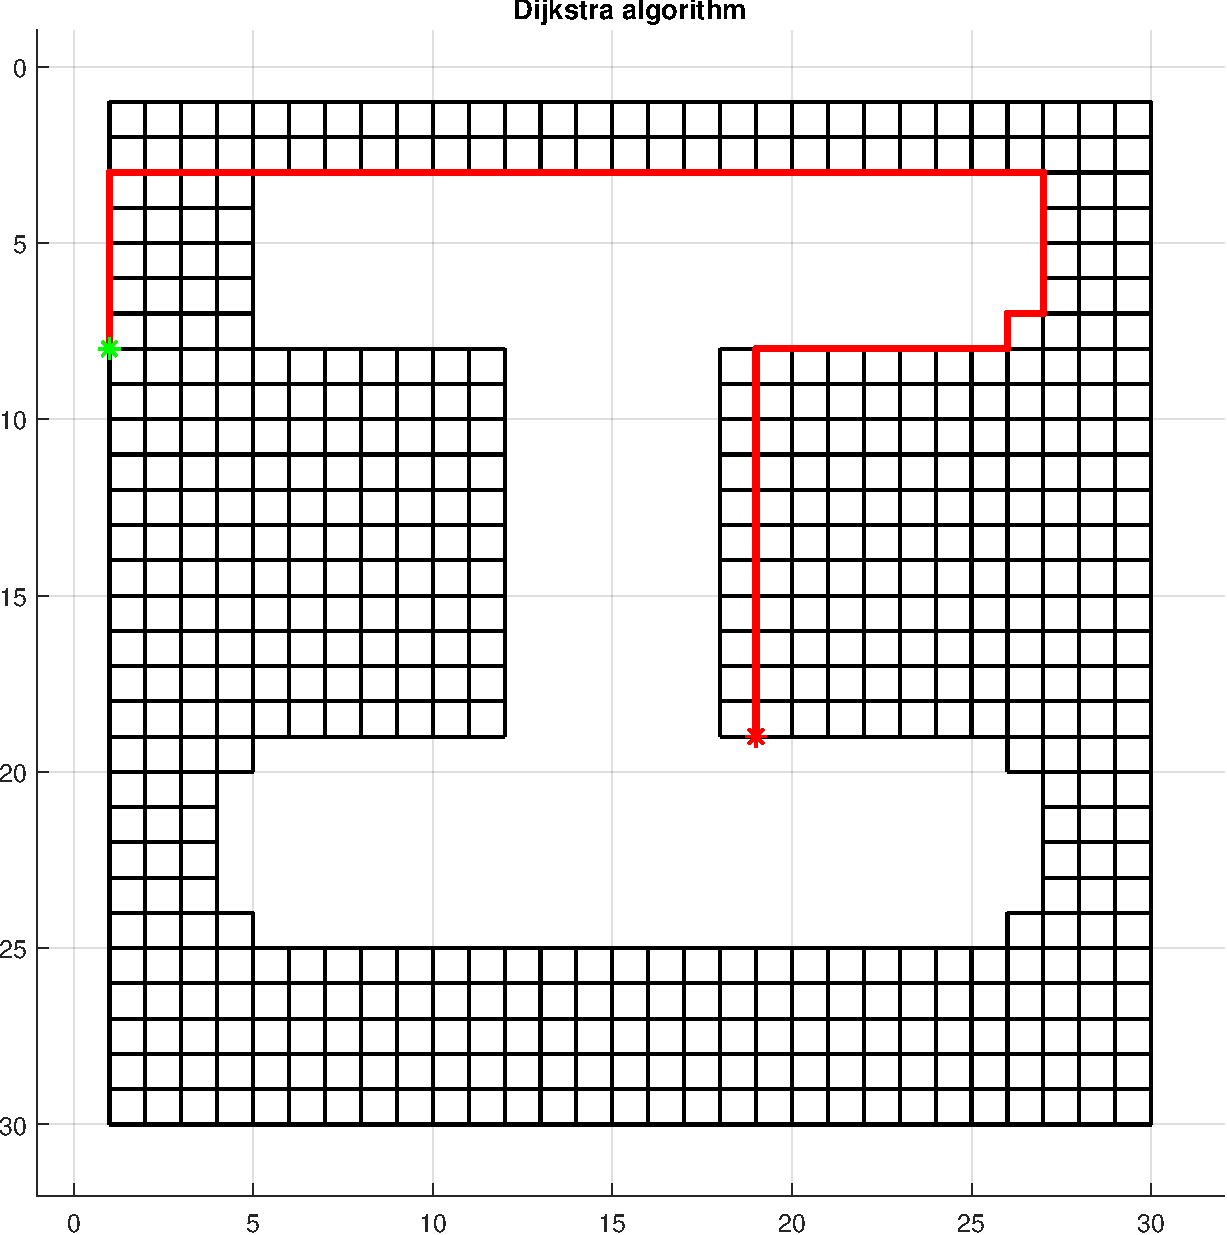
\includegraphics[width=0.48\textwidth]{./img/MATLAB/04_dijkstra_orthogonal.pdf}
    \hspace{6pt}
    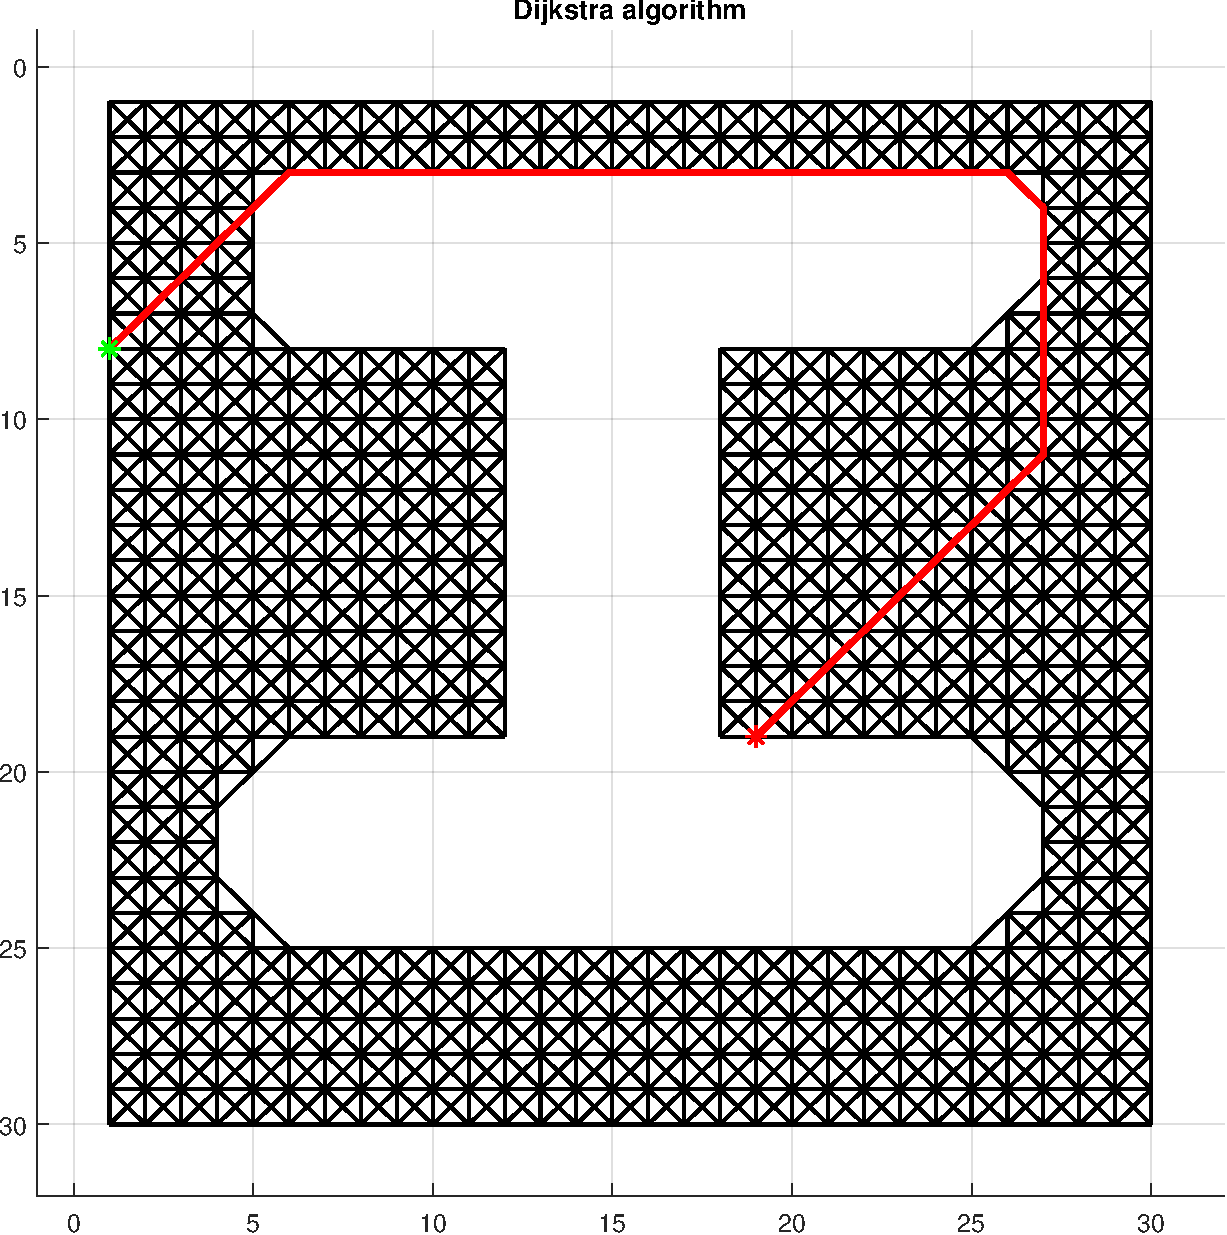
\includegraphics[width=0.48\textwidth]{./img/MATLAB/04_dijkstra_diagonal.pdf}

    \vspace{11pt}

    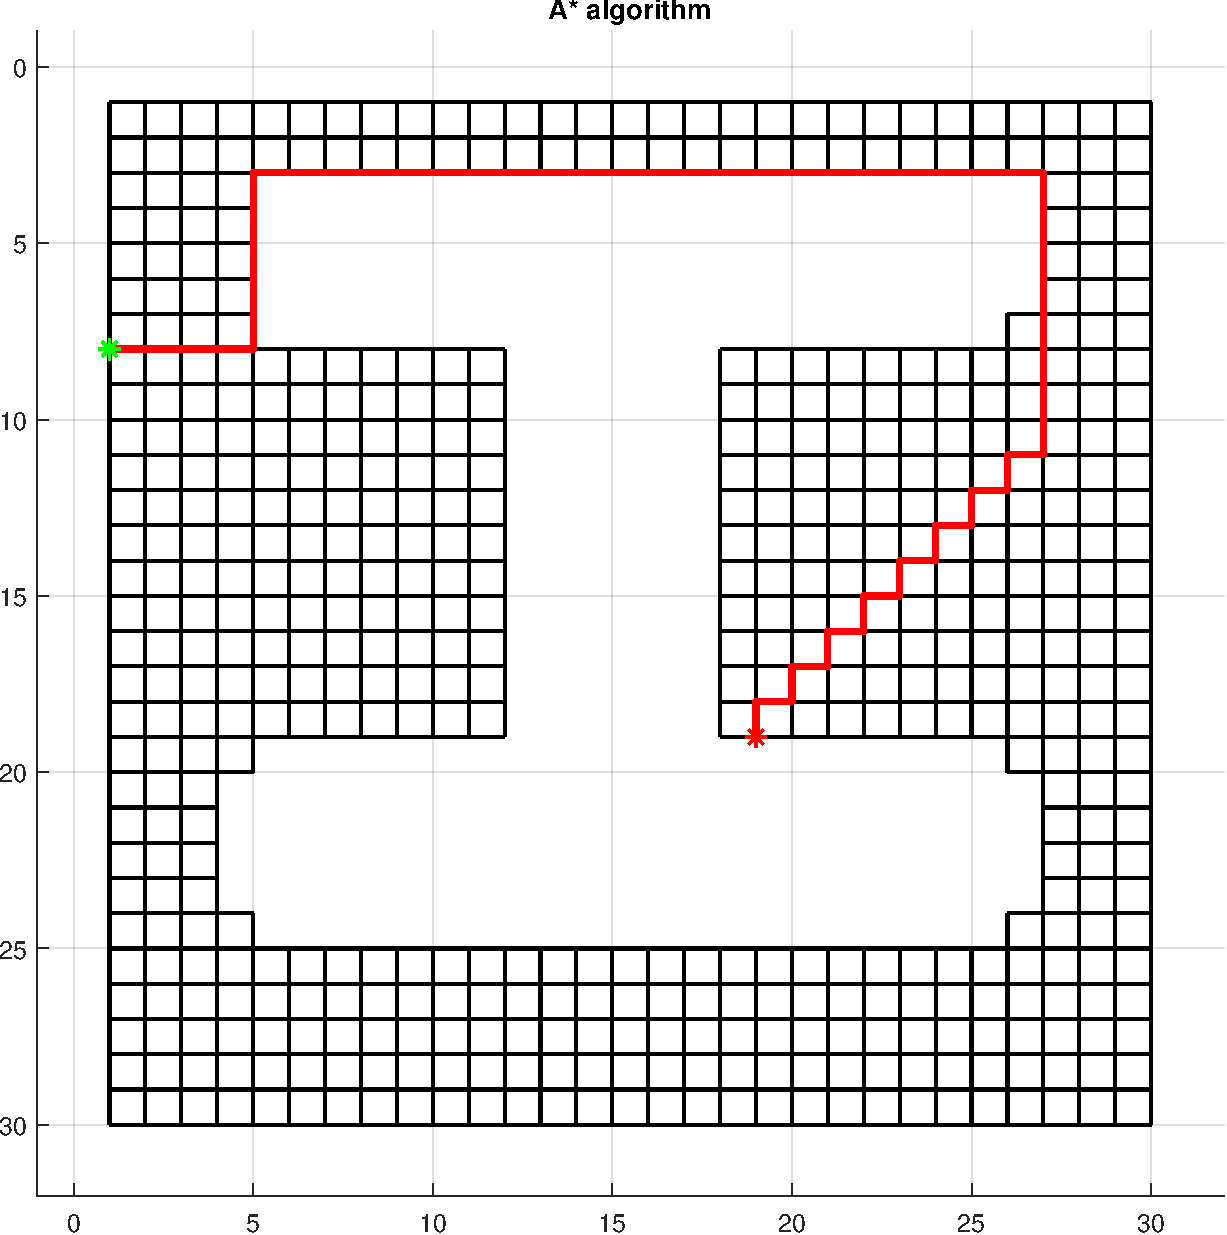
\includegraphics[width=0.48\textwidth]{./img/MATLAB/04_astar_orthogonal.pdf}
    \hspace{6pt}
    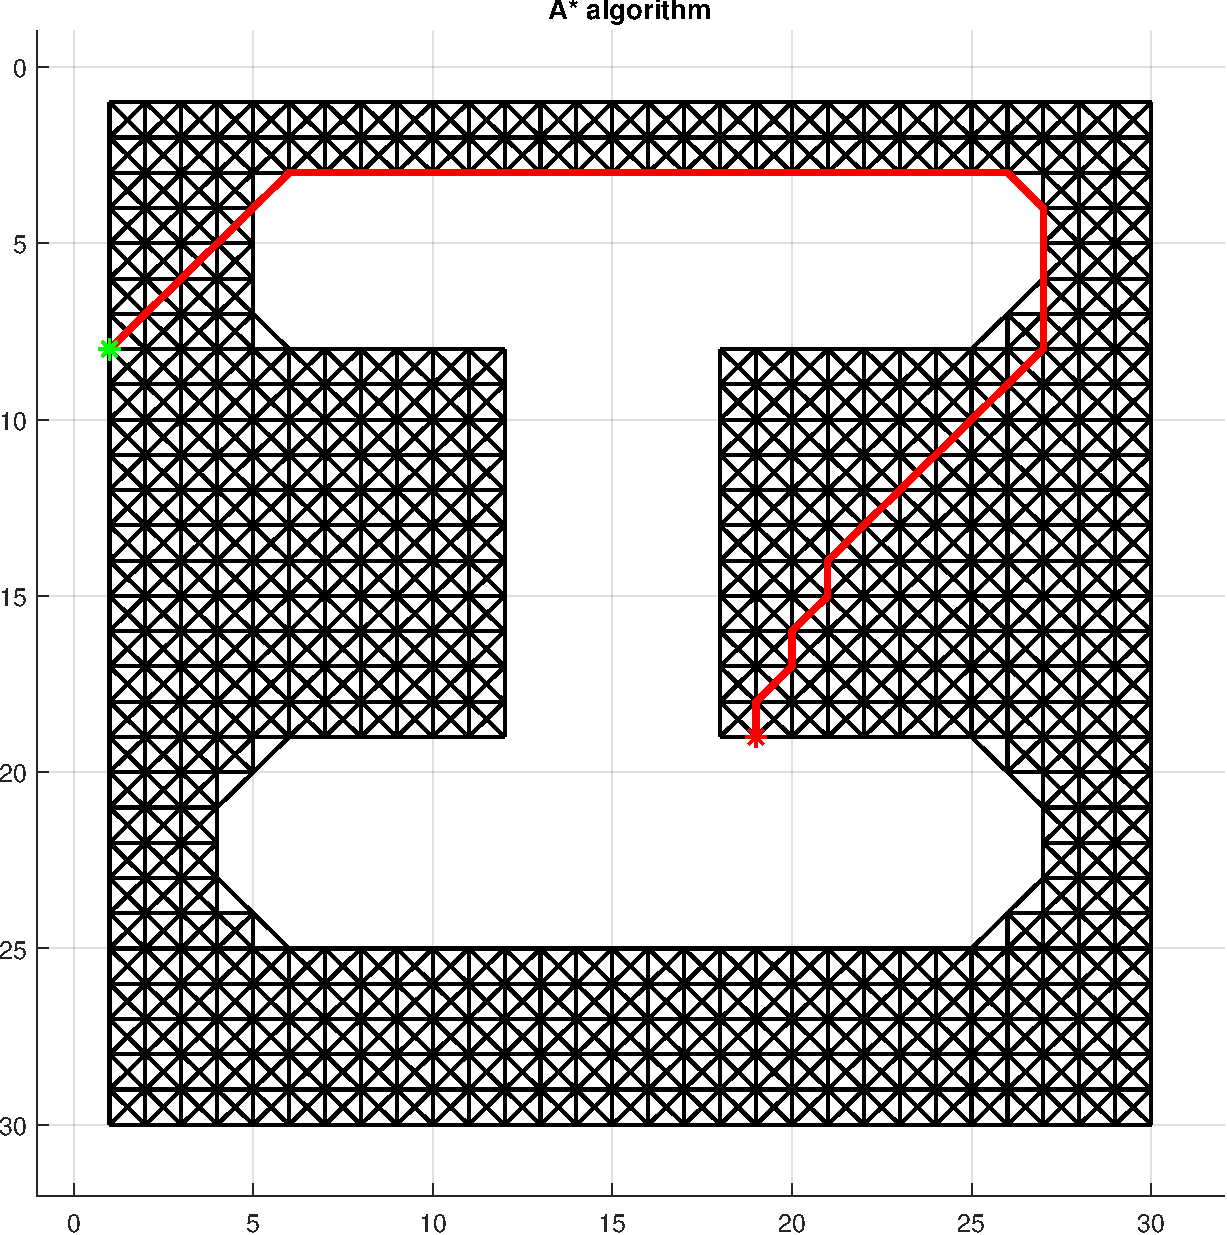
\includegraphics[width=0.48\textwidth]{./img/MATLAB/04_astar_diagonal.pdf}
    \caption{Map 4: Graph and path found by the algorithms.}
    \label{fig:map_4_results}
\end{figure}

\begin{table}[H]
    \centering
    \begin{tabular}{|c|c|c|c|c|c|}
        \hline
        \textbf{Algorithm}        & \textbf{Diagonal} & \textbf{Elapsed time (ms)} & \textbf{Nodes analyzed} & \textbf{Path length (m)} \\
        \hline
        \multirow{2}{*}{Dijkstra} & No                & 725                        & 650                     & 55                       \\
                                  & Yes               & 2799                       & 650                     & 47                       \\
        \hline
        \multirow{2}{*}{A*}       & No                & 640                        & 562                     & 55                       \\
                                  & Yes               & 2060                       & 450                     & 47                       \\
        \hline
    \end{tabular}
    \caption{Map 4: Results of the tests.}
    \label{tab:map_4_results}
\end{table}

Once again, even from the tests on Map 4, similar conclusions as before can be drawn from the results presented in Table \ref{tab:map_4_results} and in Figure \ref{fig:map_4_results}.

